\documentclass{article}

% if you need to pass options to natbib, use, e.g.:
%     \PassOptionsToPackage{numbers, compress}{natbib}
% before loading neurips_2021

% ready for submission
\usepackage[preprint]{neurips_2021}

% to compile a preprint version, e.g., for submission to arXiv, add add the
% [preprint] option:
%     \usepackage[preprint]{neurips_2021}

% to compile a camera-ready version, add the [final] option, e.g.:
%     \usepackage[final]{neurips_2021}

% to avoid loading the natbib package, add option nonatbib:
%    \usepackage[nonatbib]{neurips_2021}

\usepackage[utf8]{inputenc} % allow utf-8 input
\usepackage[T1]{fontenc}    % use 8-bit T1 fonts
\usepackage{hyperref}       % hyperlinks
\usepackage{url}            % simple URL typesetting
\usepackage{booktabs}       % professional-quality tables
\usepackage{amsfonts}       % blackboard math symbols
\usepackage{nicefrac}       % compact symbols for 1/2, etc.
\usepackage{microtype}      % microtypography
\usepackage{xcolor}         % colors

% proper quoting
\usepackage{csquotes} 

\usepackage{graphicx}



\title{Effects of Conventional and Renewable Electricity Generation on Spot Market Prices in Germany and Luxembourg}

% The \author macro works with any number of authors. There are two commands
% used to separate the names and addresses of multiple authors: \And and \AND.
%
% Using \And between authors leaves it to LaTeX to determine where to break the
% lines. Using \AND forces a line break at that point. So, if LaTeX puts 3 of 4
% authors names on the first line, and the last on the second line, try using
% \AND instead of \And before the third author name.

\author{%
Ismail Kisa\\
% Matrikelnummer \\
\texttt{ismail.kisa@student.uni-tuebingen.de}\\
\And Gereon Recht\\
% Matrikelnummer \\
\texttt{gereon.recht@student.uni-tuebingen.de} \\
  %David S.~Hippocampus\thanks{Use footnote for providing further information
   % about author (webpage, alternative address)---\emph{not} for acknowledging
   % funding agencies.} \\
  %Department of Computer Science\\
  %Cranberry-Lemon University\\
  %Pittsburgh, PA 15213 \\
  %\texttt{hippo@cs.cranberry-lemon.edu} \\
  % examples of more authors
  % \And
  % Coauthor \\
  % Affiliation \\
  % Address \\
  % \texttt{email} \\
  % \AND
  % Coauthor \\
  % Affiliation \\
  % Address \\
  % \texttt{email} \\
  % \And
  % Coauthor \\
  % Affiliation \\
  % Address \\
  % \texttt{email} \\
  % \And
  % Coauthor \\
  % Affiliation \\
  % Address \\
  % \texttt{email} \\
}

\begin{document}

\maketitle

\begin{abstract}
\begin{itemize}
    \item Increasing renewable generation in Germany $->$ EEG (Erneurbare Energien Gesetz) responsible for that
    \item This paper analyses the effect of renewabele/conventional generation on the spot market price
    \item Analyzed interval from 2019 - 2021
    \item Describe data briefly
    \item We use regression analysis
    \item Mention result: negative correlation of renewable generation and price $->$ merit-order
\end{itemize}


\end{abstract}

\section{Introduction}

\begin{itemize}
    \item explain how pricing in electricity markets works (merit order) and what spot markets are. 
    Use \citep{markets_for_electrical_energy}
    \item explain why negative prices can occur
    \item some basics about how electricity is measured (MWh)
\end{itemize}

Electricity generation can be divided into two categories: conventional and renewable. Conventional power generation refers to those power plants that require finite, fossil energy resources. These include gas, coal or oil but also nuclear power plants. On the otherside, renwable power generation uses energy sources that are continously renewed and are available unlimited. Examples are hydropower, photovoltaic, wind or biomass. Our data contains, besides the mentioned power plants, "other renewables" and "other conventionals". "Other renewables" include for example geothermal energy or landfill gas. "Other conventionals" incude trash or mineral oil. Those power plants have a small electricity generation and are merged. The most significant energies are wind and solar for renewable, and brown coal and nuclear for conventional. 

The spot market price for electricity is traded on the exchange and is determined by supply and demand. In some hours the price of electricity on the spot market is negative. This happens if high electricity generation meets low demand. In times of negative prices, the electricity generators have to pay for the acceptans of their generated electricity. 

\section{Data}
We use time series data from the years 2019 to 2021 of hourly electricity generation separated by technology type and quarter-hourly intraday spot market prices, both for the bidding zone comprised of Germany and Luxembourg \citep{smard}.
Bidding zones are areas which have the same electricity price.
We transform the spot market prices to hourly intervals by taking the mean value for each hour in order to relate them to the electricity generation data.

TODO: how is the data gathered? By TSOs?

\begin{figure}[h]
    \centering
    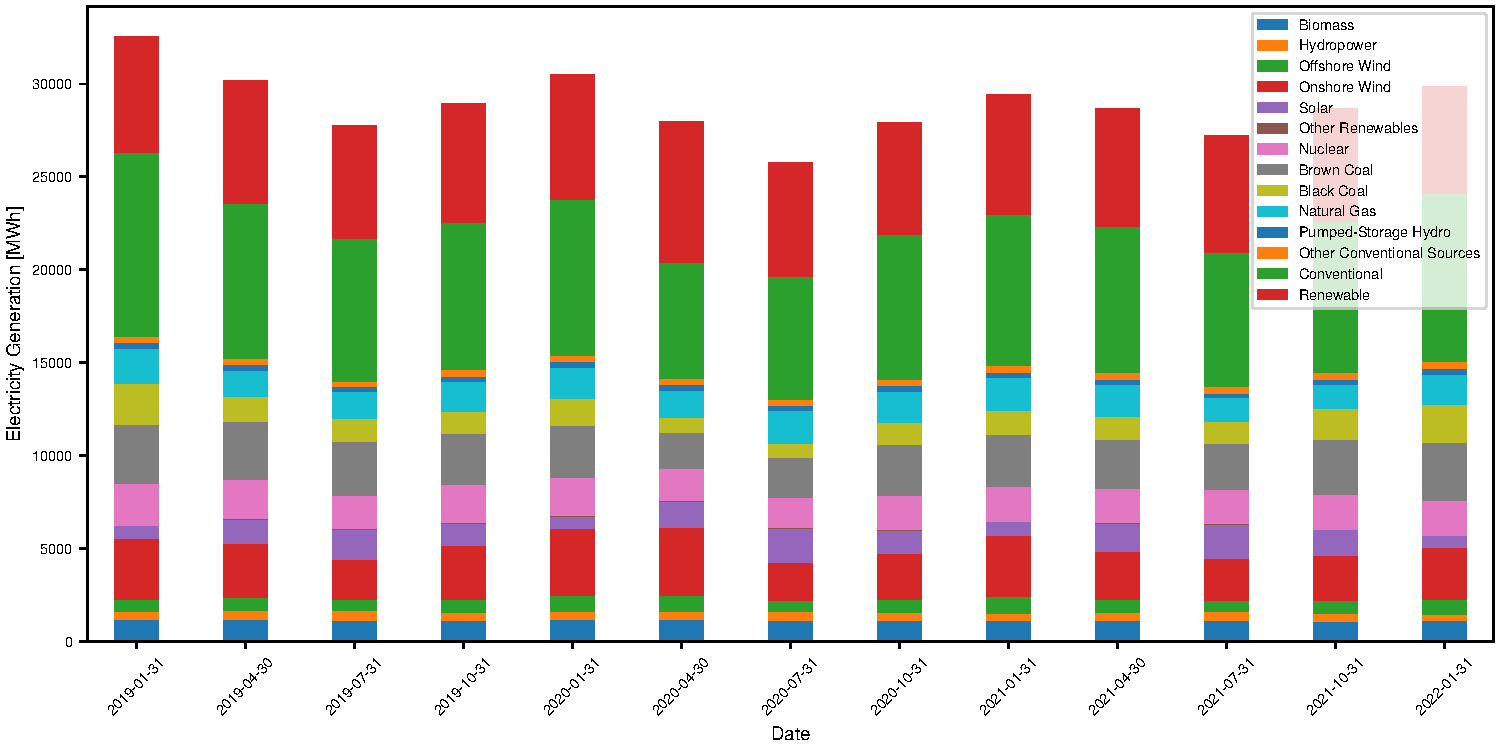
\includegraphics[width=0.8\columnwidth]{doc/fig/quarterly_technology_mix.pdf}
    \caption{Caption}
    \label{fig:quarterly_mix}
\end{figure}

\begin{itemize}
    \item Mention that pumped storage hydro is left out and analyzed seperately
    \item Mention that the price has increased a lot since 2019, while the percentage of renewable is same?
    \\
    \item Informations from \textit{https://www.smard.de/page/home/wiki-article/446/636, https://www.smard.de/page/home/wiki-article/518/562}
    \item Introduce data by showing exemplary day, maybe one where renewables depress prices
\end{itemize}

\section{Methods}

\section{Results}

\begin{itemize}
    \item Figure \ref{fig:ren_vs_con_regression} shows the opposite effects of renewable and conventional electricity generation on the prices.
    \item Data and analysis can be found on Github \citep{github_repo}.
\end{itemize}

\begin{figure}
    \centering
    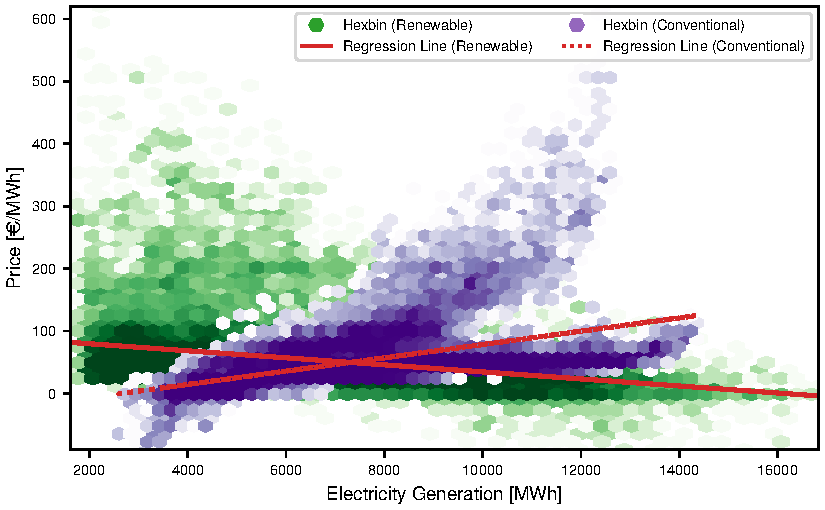
\includegraphics[width=0.7\columnwidth]{doc/fig/ren_vs_con_regression.pdf}
    \caption{Caption}
    \label{fig:ren_vs_con_regression}
\end{figure}

\begin{figure}
    \centering
    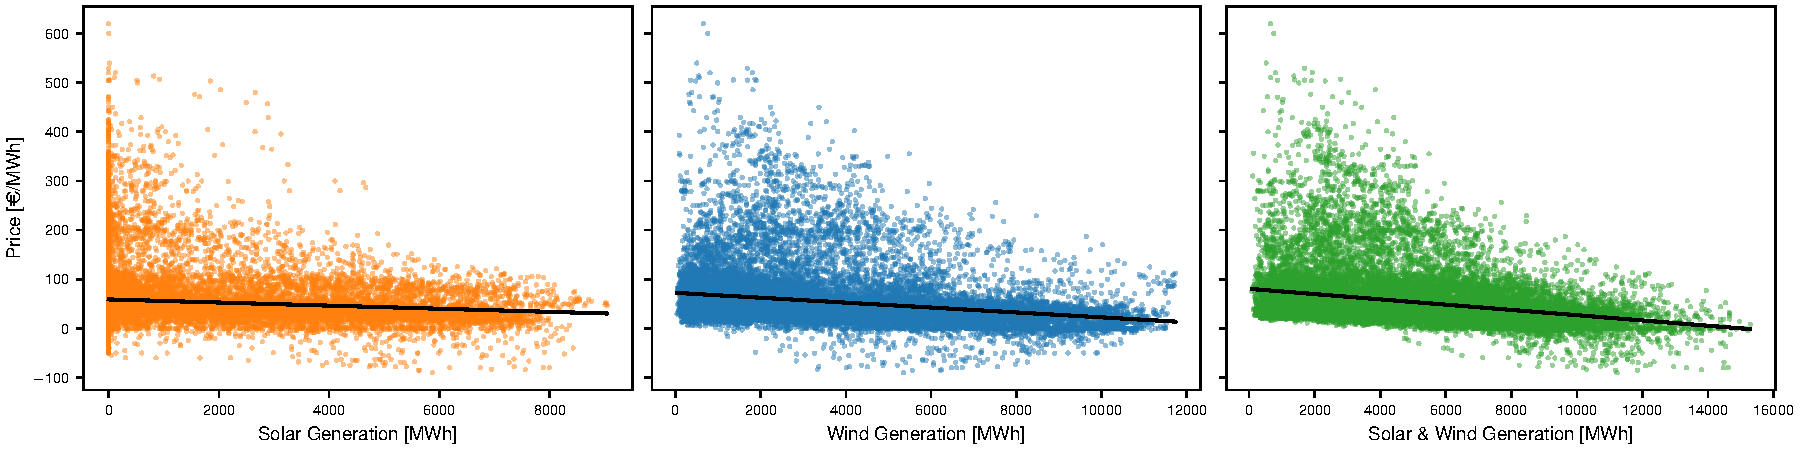
\includegraphics[width=\columnwidth]{doc/fig/solar_wind_regression.pdf}
    \caption{Caption}
    \label{fig:solar_wind_regression}
\end{figure}

\begin{figure}
    \centering
    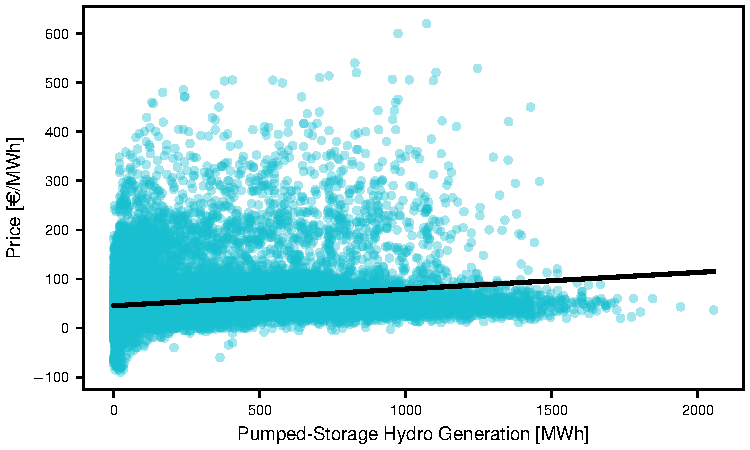
\includegraphics[width=0.7\columnwidth]{doc/fig/pumped_hydro_regression.pdf}
    \caption{Caption}
    \label{fig:pumped_hydro_regression}
\end{figure}

\section{Conclusion}

\bibliographystyle{plainnat}
\bibliography{literature}
\end{document}
